\section{\src{comp_geopot}}

\subsection{Description}

Kernel \src{comp_geopot} is taken from the original subroutine
\src{compute_geopot} in \DYNAMICO.
%
This subroutine is originally defined in module \src{caldyn_gcm_mod}.
%
This module defines subroutine \src{caldyn}, which is the main
subroutines for dynamics part of the model, and several sub-subroutines
for various terms in the governing equation, such as potential
vorticity, geopotential, etc.
%
This subroutine calculates geopotential.

\subsection{Discretization and code}

\autoref{l:definition_comp_geopot} shows the definition part of this subroutine,
and \autoref{f:pad_comp_geopot} shows the PAD of this.

\begin{LstF90}[%
caption={Definition part of \src{compute_geopot}},%
label={l:definition_comp_geopot}%
]
SUBROUTINE compute_geopot(ps,rhodz,theta, pk,geopot)
USE icosa
USE disvert_mod
USE exner_mod
USE trace
USE omp_para
IMPLICIT NONE
  REAL(rstd),INTENT(INOUT) :: ps(iim*jjm)
  REAL(rstd),INTENT(IN)    :: rhodz(iim*jjm,llm)
  REAL(rstd),INTENT(IN)    :: theta(iim*jjm,llm)    ! potential temperature
  REAL(rstd),INTENT(INOUT) :: pk(iim*jjm,llm)       ! Exner function
  REAL(rstd),INTENT(INOUT) :: geopot(iim*jjm,llm+1) ! geopotential

  INTEGER :: i,j,ij,l
  REAL(rstd) :: p_ik, exner_ik
\end{LstF90}

Where \src{ps}, \src{rhodz},
\src{theta}, \src{pk}, and \src{geopot} are
surface pressure, mass,
potential temperature, Exner function, and geopotential, respectively.
%
These arrays except \src{ps} have two dimensions,  first one is for
horizontal index and second one is for vertical index.
%
All of these are defined in the center of control volume in horizontal,
the size of first dimension is \src{iim*jjm}.
%
Also these except \src{ps} and \src{geopot} are defined in the full
level in vertical, the size of second dimension of these are \src{llm},
while \src{geopot} has the size of \src{llm+1}.

\begin{figure}[p]
\centering
 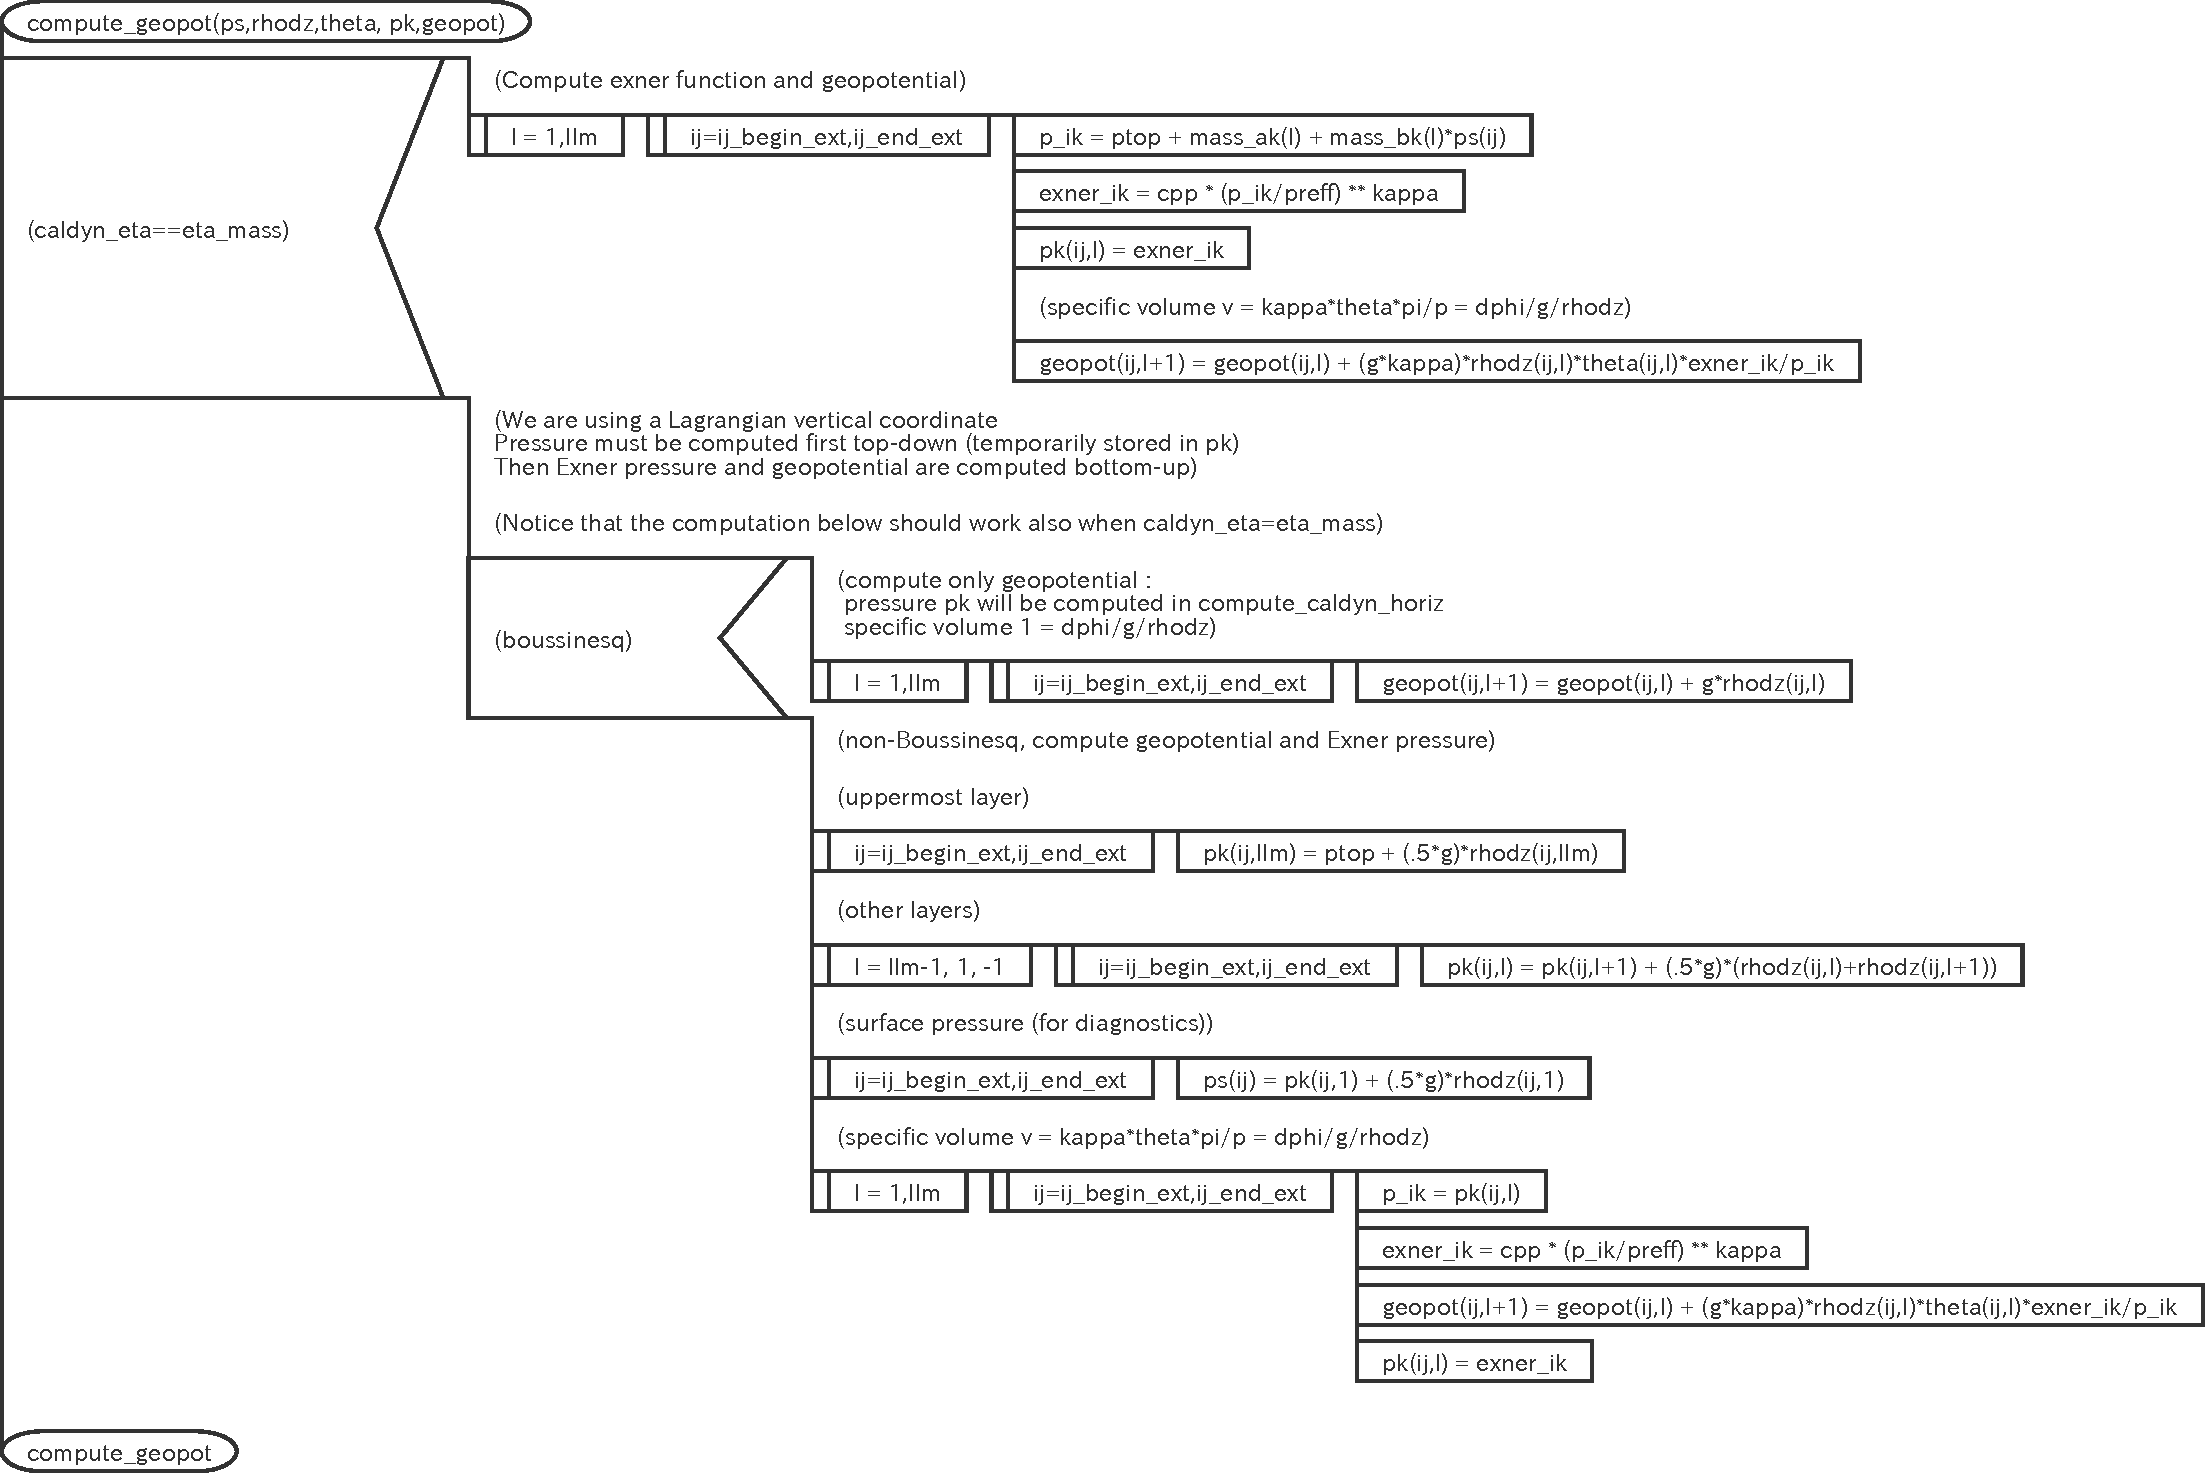
\includegraphics[scale=.45]{figs/geopot.pdf}
 \caption{PAD of \src{compute_geopot}}
 \label{f:pad_comp_geopot}
\end{figure}

Note that in this kernel package
\src{caldyn_eta} is set as \src{eta_mass},
and
\src{boussinesq} is set as \src{.true.},
so in this subroutine only \src{geopot} is calculated as

\begin{LstF90}[numbers=none]
geopot(ij,l+1) = geopot(ij,l) + g*rhodz(ij,l)
\end{LstF90}
%
and Exner pressure
are calculated in subroutine \src{compulte_caldyn_horiz}, which is also
included in this package as kernel \src{comp_caldyn_horiz}.

\clearpage



\subsection{Input data and result}

Input data file is prepared and you can download from official server using
\file{data/download.sh} script.
%
This data file is created by original \DYNAMICO\footnotemark with
Held-Suarez case parameter set included in the original source archive.
%
\footnotetext{with slight modification by AICS.}
%
Max/min/sum of input/output data of the kernel subroutine are output as
a log.
%
Below is an example of \src{$IAB_SYS=Ubuntu-gnu-ompi} case.

\begin{LstLog}
 [KERNEL] comp_geopot
 *** Start  initialize
                iim, jjm, llm:    23    25    19
             ij_begin, ij_end:    48   528
     ij_begin_ext, ij_end_ext:    24   552
             ll_begin, ll_end:     1    19
        t_right, t_rup, t_lup:     1    23    22
     t_left, t_ldown, t_rdown:    -1   -23   -22
        u_right, u_rup, u_lup:     0  1173   575
     u_left, u_ldown, u_rdown:    -1  1150   553
           z_rup, z_up, z_lup:   598     0   597
     z_ldown, z_down, z_rdown:   -23   575   -22
                   caldyn_eta:     1
                   boussinesq:     F
                            g:     9.80000000
 +check[mass_ak         ] max=  2.2205608555404415E+04,min=  2.9655441593806341E+02,sum=  1.7315769223740909E+05
 +check[mass_bk         ] max=  9.8820601234384886E-01,min=  0.0000000000000000E+00,sum=  6.4254510678414123E+00
 *** Finish initialize
 *** Start kernel
 ### check point iteration:        1000
 ### Input ###
 +check[ps_prev         ] max=  1.0000000000000000E+05,min=  1.0000000000000000E+05,sum=  5.7500000000000000E+07
 +check[rhodz           ] max=  1.2306877011993038E+03,min=  0.0000000000000000E+00,sum=  5.3979591836733194E+06
 +check[theta           ] max=  8.0139914420291746E+02,min=  0.0000000000000000E+00,sum=  3.8582633571973117E+06
 +check[pk_prev         ] max=  1.0014594722514462E+03,min=  0.0000000000000000E+00,sum=  6.9872296819747351E+06
 +check[geopot_prev     ] max=  3.8250620498369227E+05,min=  0.0000000000000000E+00,sum=  1.1718001851963627E+09
 ### Output ###
 +check[ps              ] max=  1.0000000000000000E+05,min=  1.0000000000000000E+05,sum=  5.7500000000000000E+07
 +check[pk              ] max=  1.0014594722514462E+03,min=  0.0000000000000000E+00,sum=  6.9872296819747351E+06
 +check[geopot          ] max=  3.8250620498369227E+05,min=  0.0000000000000000E+00,sum=  1.1718001851963627E+09
 ### final iteration:        1000
 ### Validation : grid-by-grid diff ###
 +check[ps              ] max=  0.0000000000000000E+00,min=  0.0000000000000000E+00,sum=  0.0000000000000000E+00
 +check[pk              ] max=  0.0000000000000000E+00,min=  0.0000000000000000E+00,sum=  0.0000000000000000E+00
 +check[geopot          ] max=  0.0000000000000000E+00,min=  0.0000000000000000E+00,sum=  0.0000000000000000E+00
 *** Finish kernel
\end{LstLog}

Check the lines below \src{``Validation : grid-by-grid diff''} line,
that shows difference between calculated output array and
pre-calculated reference array.
These should be zero or enough small to be acceptable.
%
There are sample output log files in \file{reference/}
in each kernel program directory, for reference purpose.

\subsection{Sample of performance result}

Here's an example of the performance result part of the log output.
Below is an example executed with the machine environment described in \autoref{s:measuring_env}.
%
Note that in this program kernel part is iterated 1000 times.

\begin{LstLog}
 *** Computational Time Report
 *** ID=001 : MAIN_comp_geopot                 T=     0.824 N=   1000
\end{LstLog}
